\documentclass[10pt]{article}
\usepackage{amsmath}
\usepackage{amsfonts}
\usepackage{amssymb}
\usepackage{tikz,multicol}
\usetikzlibrary{decorations.text}

\usepackage[utf8]{vietnam}
\usepackage[left=2cm,right=2cm,top=1cm,bottom=1.5cm]{geometry}
\begin{document}
	\centering \fontsize{16pt}{2pt}\selectfont\textbf{ĐẶT ĐỘ DÀI TRONG TIKZ}
	
	\textbf{HỒ HÀ ĐẶNG}\footnote{Nhóm Toán và \LaTeX}
	\section*{Đặt độ dài 1 đoạn thẳng}
	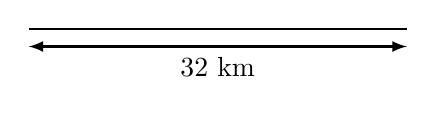
\begin{tikzpicture}[>=latex,thick,scale=1.5]
		\coordinate (a) at (0,0);
		\coordinate (b) at (3.2,0);
		\draw (a) -- (b);
		\draw[<->] ([yshift=-0.15cm]a) -- ([yshift=-0.15cm]b) node[midway, below]{32 km};
	\end{tikzpicture}
	
	\section*{Đặt độ dài nhiều đoạn thẳng}	
	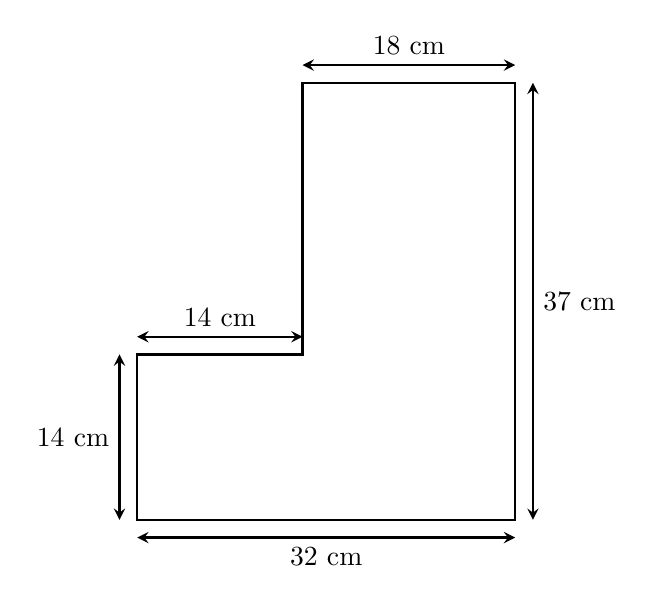
\begin{tikzpicture}[>=stealth,thick,scale=1.5]
		% set up coordinates for an easy use
		\coordinate (a) at (0,0);
		\coordinate (b) at (3.2,0);
		\coordinate (c) at (3.2,3.7);
		\coordinate (d) at ({3.2-1.8},3.7);
		\coordinate (e) at (1.4,1.4);
		\coordinate (f) at (0,1.4);
		\draw (a) -- (b) -- (c) -- (d) -- (e) -- (f) -- cycle;
		\draw[<->] ([yshift=-0.15cm]a) -- ([yshift=-0.15cm]b) node[midway, below]{32 cm};
		\draw[<->] ([xshift=+0.15cm]b) -- ([xshift=+0.15cm]c) node[midway, right]{37 cm};
		\draw[<->] ([yshift=+0.15cm]c) -- ([yshift=+0.15cm]d) node[midway, above]{18 cm};
		\draw[<->] ([yshift=+0.15cm]e) -- ([yshift=+0.15cm]f) node[midway, above]{14 cm};
		\draw[<->] ([xshift=-0.15cm]f) -- ([xshift=-0.15cm]a) node[midway, left]{14 cm};
	\end{tikzpicture}
	\section*{Đặt độ dài đường thẳng và chéo}
	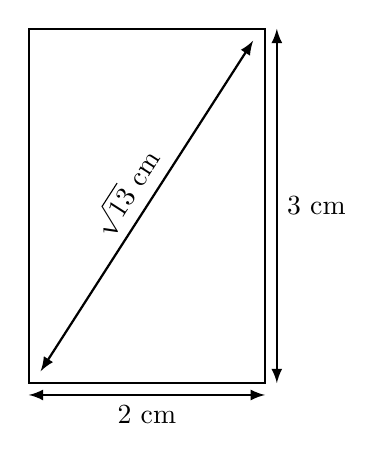
\begin{tikzpicture}[>=latex,thick,scale=1.5]
		% set up coordinates for an easy use
		\coordinate (a) at (0,0);
		\coordinate (b) at (2,0);
		\coordinate (c) at (2,3);
		\coordinate (d) at (0,3);
		\draw (a) -- (b) -- (c) -- (d)-- cycle;
		\draw[<->] ([yshift=-0.1cm]a) -- ([yshift=-0.1cm]b) node[midway, below]{2 cm};
		\draw[<->] ([xshift=+0.1cm]b) -- ([xshift=+0.1cm]c) node[midway, right]{3 cm};
		\draw[<->] ([xshift=+0.1cm,yshift=+0.1cm]a) -- ([xshift=-0.1cm,yshift=-0.1cm]c) node[midway, sloped, above]{$ \sqrt{13} $ cm};
		%\draw[<->] ([yshift=+0.15cm]e) -- ([yshift=+0.15cm]f) node[midway, above]{14 cm};
		%\draw[<->] ([xshift=-0.15cm]f) -- ([xshift=-0.15cm]a) node[midway, left]{14 cm};
	\end{tikzpicture}
	\newpage
	\section*{Đặt độ dài đường tròn}
	\begin{multicols}{2}
		\textbf{Công thức toán không bẻ cong được}
		
		\begin{tikzpicture}[scale=.8]
			\draw (0,0)--(2,0) node[above]{$ 5 $ cm}--(4,0);
			\draw[blue]
			(4cm,0) arc [start angle=0,end angle=90,radius=4cm];
			\draw[<->,blue]
			(4cm+2mm,0) arc [start angle=0,end angle=90,radius=4cm+2mm];
			\draw[blue]
			(4cm,0) arc [start angle=0,end angle=90,radius=4cm];
			\draw[blue,dashed]
			(4cm,0) arc [start angle=0,end angle=-270,radius=4cm];
			\path[decorate,decoration={text along path,
				text={${\dfrac{2\times5\times\pi}{4}}$cm},text align=center}]
			(0,5cm) arc [start angle=-270,end angle=-360,radius=5cm];
		\end{tikzpicture}
		
		\textbf{Chỉ có thể bẻ cong text}
		
		\begin{tikzpicture}[scale=.8]
			\draw (0,0)--(2,0) node[above]{$ r $ cm}--(4,0);
			\draw[blue]
			(4cm,0) arc [start angle=0,end angle=90,radius=4cm];
			\draw[<->,blue]
			(4cm+2mm,0) arc [start angle=0,end angle=90,radius=4cm+2mm];
			\draw[blue]
			(4cm,0) arc [start angle=0,end angle=90,radius=4cm];
			\draw[blue,dashed]
			(4cm,0) arc [start angle=0,end angle=-270,radius=4cm];
			\path[decorate,decoration={text along path,
				text={$d$/4 cm},text align=center}]
			(0,4cm+6mm) arc [start angle=-270,end angle=-360,radius=4cm+6mm];
		\end{tikzpicture}
	\end{multicols}
	\section*{Đặt độ dài đường elip}
	\begin{tikzpicture}[scale=2]
		\draw (0,0)--(2,0) node[above]{\small$ a $ cm}--(4,0);
		\draw (0,0)--(0,1) node[left]{\small $ b $ cm}--(0,2);
		\draw[blue]
		(4cm,0) arc [start angle=0,end angle=90,x radius=4cm, y radius=2cm];
		\draw[<->,blue]
		(4cm+2mm,0) arc [start angle=0,end angle=90,x radius=4cm+2mm, y radius=2cm+2mm];
		\draw[blue]
		(4cm,0) arc [start angle=0,end angle=90,x radius=4cm, y radius=2cm];
		\draw[blue,dashed]
		(4cm,0) arc [start angle=0,end angle=-270,x radius=4cm, y radius=2cm];
		\path[decorate,decoration={text along path,
			text={${\dfrac{d}{4}}$ cm},text align=center}]
		(0,2.4cm) arc [start angle=-270,end angle=-360,x radius=4.5cm, y radius=2.5cm];
	\end{tikzpicture}
	
\end{document}